\documentclass{beamer}

\usepackage{listings}
\usepackage{graphicx}
\usepackage{wrapfig}
\usepackage{tikz}
\usepackage{pgfplots}
\usepackage{stmaryrd}
\usepackage{mathptmx}
\usepackage{anyfontsize}
\usepackage{t1enc}
\usepackage{color}
\usetikzlibrary{arrows.meta}
\usetikzlibrary{calc}
\setbeamersize{text margin left=2mm,text margin right=30mm} 
\beamertemplatenavigationsymbolsempty
\newcommand{\icol}[1]{
  \left(\begin{smallmatrix}#1\end{smallmatrix}\right)
}

\lstnewenvironment{casepython}
{
	\renewcommand\lstlistingname{CasePython}
	\lstset{style = mystylepython}
}{}

\lstnewenvironment{casecplusplus}
{
	\renewcommand\lstlistingname{CaseCPlusPlus}
	\lstset{style = mystylecplusplus}
}{}

\lstset % why no line numbers (not in frame ?)
{
    frame=tb,
    tabsize=4,
    showstringspaces=false,
    numbers=left,
    commentstyle=\color{gray},
    keywordstyle=\color{blue},
    stringstyle=\color{red},
		literate=
		{á}{{\'a}}1 {é}{{\'e}}1 {í}{{\'i}}1 {ó}{{\'o}}1 {ú}{{\'u}}1
    {Á}{{\'A}}1 {É}{{\'E}}1 {Í}{{\'I}}1 {Ó}{{\'O}}1 {Ú}{{\'U}}1
    {à}{{\`a}}1 {è}{{\`e}}1 {ì}{{\`i}}1 {ò}{{\`o}}1 {ù}{{\`u}}1
    {À}{{\`A}}1 {È}{{\'E}}1 {Ì}{{\`I}}1 {Ò}{{\`O}}1 {Ù}{{\`U}}1
    {ä}{{\"a}}1 {ë}{{\"e}}1 {ï}{{\"i}}1 {ö}{{\"o}}1 {ü}{{\"u}}1
    {Ä}{{\"A}}1 {Ë}{{\"E}}1 {Ï}{{\"I}}1 {Ö}{{\"O}}1 {Ü}{{\"U}}1
    {â}{{\^a}}1 {ê}{{\^e}}1 {î}{{\^i}}1 {ô}{{\^o}}1 {û}{{\^u}}1
    {Â}{{\^A}}1 {Ê}{{\^E}}1 {Î}{{\^I}}1 {Ô}{{\^O}}1 {Û}{{\^U}}1
    {œ}{{\oe}}1 {Œ}{{\OE}}1 {æ}{{\ae}}1 {Æ}{{\AE}}1 {ß}{{\ss}}1
    {ç}{{\c c}}1 {Ç}{{\c C}}1 {ø}{{\o}}1 {å}{{\r a}}1 {Å}{{\r A}}1
    {€}{{\EUR}}1 {£}{{\pounds}}1
}

\lstdefinestyle{mystylepython}
{
    language = Python,
		otherkeywords = {},
}

\lstdefinestyle{mystylecplusplus}
{
    language = C++,
		otherkeywords = {},
}

%\def\FunctionF(#1){(#1)^4 + 5*(#1)^3 - 10*(#1)} will cause problems
\def\FunctionF(#1){(#1)^4 - 3*(#1)^3}
% machine learning supervisé

\begin{document}

	\title{Descente de gradient stochastique}
	\date{}
	\maketitle

	\newpage
	
	\begin{wrapfigure}{r}{0.5\linewidth}
	\centering
			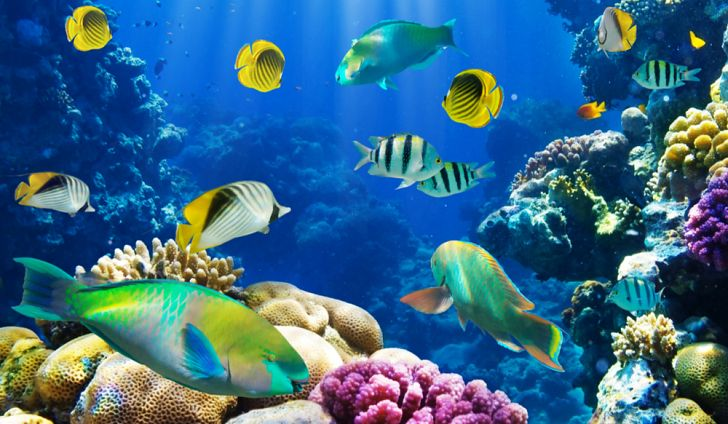
\includegraphics[width=100pt]{pictures/fish.jpg}
		\caption{Entrée: photo de différentes espèces de poissons}
	\end{wrapfigure}
	
		\begin{wrapfigure}{l}{0.5\linewidth}
	\centering
			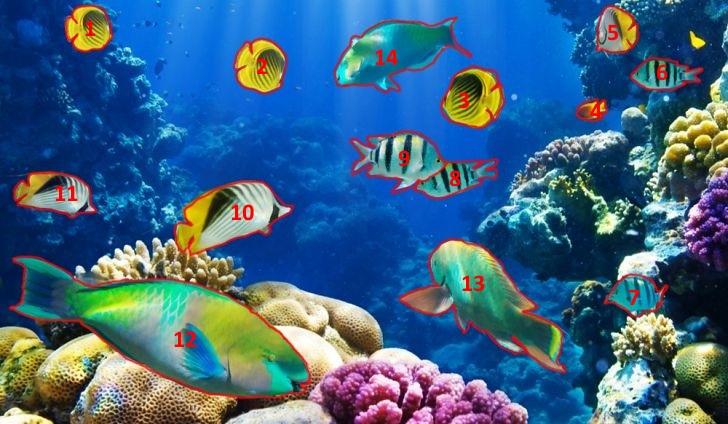
\includegraphics[width=160pt]{pictures/fishAll.jpg}
		\caption{Sortie: analyse de la photo}
	\end{wrapfigure}
	
	\raggedright\hspace{0.7cm}Sortie:\\
	\hspace{0.6cm}- 1, 2, 3: espèce 1\\
	\hspace{0.6cm}- 4: espèce 2\\
	\hspace{0.6cm}- 5: espèce 3\\
	\hspace{0.6cm}- 6, 7, 8 et 9: espèce 4\\
	\hspace{0.6cm}- 10, 11: espèce 5\\
	\hspace{0.6cm}- 12, 13, 14: espèce 6
					
	\newpage
	
	\begin{tikzpicture}
\begin{axis}[
        axis y line=center,
        axis x line=middle, 
        axis on top=true,
        xmin=-3.5,
        xmax=4.5,
        ymin=-15,
        ymax=45,
        height=11.0cm,
        width=11.0cm,
        grid,
        xtick={-3,...,4},
        ytick={-15,-10,...,40},
    ]
    \addplot [domain=-3:4, samples=50, mark=none, ultra thick, blue] {\FunctionF(x)};
    \node [left, blue] at (axis cs: 3.6,42) {$x^4-3x^3$};
		
		\coordinate (M0) at (700, 36.44);
		\node (M00) at ([shift=({0.3cm,0.3cm})]M0) {$M_0$};
		\node at (M0)[green, circle, fill, inner sep=1.5pt]{};
		
		\coordinate (M1) at (675, 23.58);
		\node (M10) at ([shift=({0.4cm,0.3cm})]M1) {$M_1$};
		\node (A0) at ([shift=({0.5cm,1.2cm})]M1) {$\alpha$};
		\node at (M1)[green, circle, fill, inner sep=1.5pt]{};
		
		\coordinate (M2) at (635, 11.53);
		\node (M20) at ([shift=({0.3cm,-0.3cm})]M2) {$M_2$};
		\node (A1) at ([shift=({0.6cm,1.2cm})]M2) {$\alpha$};
		\node at (M2)[green, circle, fill,inner sep=1.5pt]{};
		
		\draw[red,ultra thick,-{Latex[length=5mm, width=2mm]}] (M0) -- (M1);
		\draw[red,ultra thick,-{Latex[length=5mm, width=2mm]}] (M1) -- (M2);
		
\end{axis}
\end{tikzpicture}

\newpage

\begin{tikzpicture}
\begin{axis}[
        axis y line=center,
        axis x line=middle, 
        axis on top=true,
        xmin=-3.5,
        xmax=4.5,
        ymin=-15,
        ymax=45,
        height=11.0cm,
        width=11.0cm,
        grid,
        xtick={-3,...,4},
        ytick={-15,-10,...,40},
    ]
    \addplot [domain=-3:4, samples=50, mark=none, ultra thick, blue] {\FunctionF(x)};
    \node [left, blue] at (axis cs: 3.6,42) {$x^4-3x^3$};
		
		\coordinate (M0) at (700, 36.44);
		\node (M00) at ([shift=({0.3cm,0.3cm})]M0) {$M_0$};
		\node at (M0)[green, circle, fill, inner sep=1.5pt]{};
		
		\coordinate (M1) at (675, 23.58);
		\node (M10) at ([shift=({0.4cm,0.3cm})]M1) {$M_1$};
		\node at (M1)[green, circle, fill, inner sep=1.5pt]{};
		
		\coordinate (M2) at (635, 11.53);
		\node (M20) at ([shift=({0.3cm,-0.3cm})]M2) {$M_2$};
		\node (M40) at ([shift=({0.3cm,-0.7cm})]M2) {$M_4$};
		\node (MX0) at ([shift=({0.3cm,-1.1cm})]M2) {$...$};
		\node at (M2)[green, circle, fill,inner sep=1.5pt]{};
		
		\coordinate (M3) at (441, 13.53);
		\node (M30) at ([shift=({0.3cm,0.3cm})]M3) {$M_3$};
		\node (M50) at ([shift=({0.3cm,0.7cm})]M3) {$M_5$};
		\node (MX0) at ([shift=({0.3cm,1.1cm})]M3) {$...$};
		\node at (M3)[green, circle, fill,inner sep=1.5pt]{};
		
\end{axis}
\end{tikzpicture}

	\newpage
	
	\vspace*{\fill}
	Taux d'apprentissage:
\LARGE$\forall n \in \mathbb{N}, \alpha_n = \frac{1}{n + 1}$
\vspace*{\fill}

\newpage

\begin{figure}
	\centering
			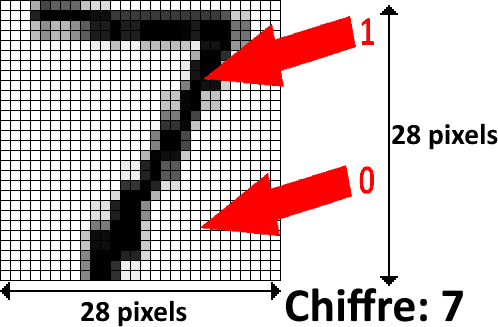
\includegraphics[width=150pt]{pictures/mnist.png}
		\caption{Exemple d'élément de MNIST annoté}
	\end{figure}
	
\normalsize A $n$ fixé avec $n \in \llbracket 0; 9\rrbracket$.
{\fontsize{6}{7}\selectfont
\begin{center}
	\begin{tabular}{ |c||c|c|c|c|c|c| } 
	 \hline
	 Sortie & 0 & 0.1 & ... & 0.9 & 1 &\\ 
	\hline
	 L'image & ne correspond pas & ne semble pas correspondre & ... & semble correspondre & correspond & à un $n$\\
	 \hline
	\end{tabular}
\end{center}}

	\newpage
	
	\normalsize
	A $n$ fixé avec $n \in \llbracket 0; 9\rrbracket$.
	
	\vspace{0.3cm}Notations: $\alpha$ est le taux d'apprentissage.\\
	On pose $m$ le nombre de photos.\\
	Soit $j \in \llbracket 1; 28^2 \rrbracket, \theta_j$ est le $j$-ème paramètre définissant la droite passant au plus près des points.\\
	$h_\theta(x^{(i)})$ est la prédiction de notre algorithme pour la $i$-ème photo $x^{(i)}$.\\
	$y^{(i)}$ vaut 0 ou 1, 1 si la photo correspond à un $n$ et 0 sinon.
	
	\vspace{0.3cm}On a $h_\theta(x^{(i)}) = \sigma(\theta_1 + \theta_2 x_2 + ... + \theta_{28^2} x_{28^2})$, avec $\sigma$ la fonction bijective sigmoïde de $\mathbb{R}$ dans [0; 1], définie par: $\sigma(x) = \frac{1}{1 + e^{-x}}$
	
	\vspace{0.3cm}On pose la fonction de coût: $J(\theta_1, \theta_2, ..., \theta_{28^2}) = \frac{1}{2m}\sum_{i=1}^{m}(h_\theta(x^{(i)}) - y^{(i)})^2$
	
	\vspace{0.3cm}Répétez tant que cela converge:\\
	Pour $j$ allant de 1 à $28^2$:\\
	$\theta_j := \theta_j - \alpha\frac{dJ(\theta_1, \theta_2, ... \theta_{28^2})}{d\theta_j}$%\frac{\alpha}{m}\sum_{i=1}^{m}(h_{\theta}(x^{(i)}) - y^{(i)}) * x_j^{(i)}$
	
	\newpage
	
	Soit $j \in \llbracket 1; 28^2 \rrbracket$.\\
	On a:\\
	$\frac{dJ(\theta_1, \theta_2, ... \theta_{28^2})}{d\theta_j} = \frac{d}{d\theta_j}(\frac{1}{2m}\sum_{i=1}^{m}(h_\theta(x^{(i)})^2 - 2 h_\theta(x^{(i)}) y^{(i)} + {y^{(i)}}^2))$\\
	= $\frac{d}{d\theta_j}(\frac{1}{2m}\sum_{i=1}^{m}(h_\theta(x^{(i)})^2 - 2 h_\theta(x^{(i)}) y^{(i)}))$ car $y^{(i)}$ est constant.\\
	= $\frac{1}{2m}\sum_{i=1}^{m}2h_\theta(x^{(i)})\frac{dh_\theta(x^{(i)})}{d\theta_j} - 2 \frac{dh_\theta(x^{(i)})}{d\theta_j} y^{(i)}$\\
	= $\frac{1}{m}\sum_{i=1}^{m}\frac{dh_\theta(x^{(i)})}{d\theta_j}(h_\theta(x^{(i)}) - y^{(i)})$\\
	
	\vspace{0.3cm}$\forall i \in \llbracket 1; m \rrbracket$, on a $\frac{dh_\theta(x^{(i)})}{d\theta_j} = \frac{d(\theta_1 x_1 + ... + \theta_{28^2} x_{28^2}))}{d\theta_j} * \frac{1}{1+e^{-(\theta_1 x_1 + ... + \theta_{28^2} x_{28^2})}} = \frac{x_i}{1 + e^{-(\theta_1 x_1 + ... + \theta_{28^2} x_{28^2})}}$ par dérivée de composition.\\
	
	\vspace{0.3cm}D'où: $\frac{dJ(\theta_1, \theta_2, ... \theta_{28^2})}{d\theta_j} = \frac{1}{m}\sum_{i=1}^{m} \frac{x_i (h_\theta(x^{(i)}) - y^{(i)})}{1 + e^{-(\theta_1 x_1 + ... + \theta_{28^2} x_{28^2})}}$

	\newpage

	\tiny
\begin{casepython}
from os import chdir as cd
from pickle import load
from math import sqrt, exp
from random import random
import gzip
from copy import deepcopy

cd("MNIST-dataset")

ft = gzip.open('data_training', 'rb')
TRAINING = load(ft)
OLD_TRAINING = deepcopy(TRAINING[1])
ft.close()

NB_ELEMENTS = len(TRAINING[0])
THETA_NUMBER = int(len(TRAINING[0][0]))
SIZE = int(sqrt(THETA_NUMBER))
STEP = 0.02 / NB_ELEMENTS

theta = [[0] * THETA_NUMBER for i in range(10)]
newTheta = [[0] * THETA_NUMBER for i in range(10)]
H_THETA = [[0] * NB_ELEMENTS for i in range(10)]
E_MY_SUM = [[0] * NB_ELEMENTS for i in range(10)]
NEW_TRAINING = [[int(OLD_TRAINING[pic] != nb) for pic in range(NB_ELEMENTS)] for nb in range(10)]

def mySum(picIndex, numberIndex):
    partialSum = 0
    for j in range(THETA_NUMBER):
        partialSum += theta[numberIndex][j] * TRAINING[0][picIndex][j]
    return partialSum

def h_theta(picIndex, numberIndex):
    partialSum = 0
    for i in range(1, THETA_NUMBER):
        partialSum += theta[numberIndex][i] * TRAINING[0][picIndex][i]
    return theta[numberIndex][0] + partialSum

def dh_theta(picIndex, thetaIndex, numberIndex):
    return TRAINING[0][picIndex][thetaIndex] / (1 + E_MY_SUM[numberIndex][picIndex])

def prediction(index):
    bestIndex = -1
    bestDistance = 10 # "largest" distance
    for numberIndex in range(10):
        hTet = h_theta(index, numberIndex)
        if hTet < bestDistance:
            bestIndex = numberIndex
            bestDistance = hTet
    return bestIndex

def predictionRate():
    nb = 0
    for i in range(NB_ELEMENTS):
        if OLD_TRAINING[i] == prediction(i): nb += 1
    print((nb / NB_ELEMENTS) * 100, nb, NB_ELEMENTS)

def predictionIndex(index):
    prediction = 0
    nbIndex = 0
    for i in range(NB_ELEMENTS):
        if OLD_TRAINING[i] == index:
            nbIndex += 1
            if not bool(round(h_theta(i, index))):
                prediction += 1
    return prediction

for numberIndex in range(10):
    print(numberIndex)

    iteration = 0
    lastValue = NB_ELEMENTS
    predi = predictionIndex(numberIndex)
    lastImprove = 0
    while predi <= lastValue and lastImprove < 2:
        if predi == lastValue: lastImprove += 1
        else: lastImprove = 0
        lastValue = predi
        print("iteration", iteration, predi)
        
        for k in range(NB_ELEMENTS):
            H_THETA[numberIndex][k] = h_theta(k, numberIndex)
            E_MY_SUM[numberIndex][k] = exp(-mySum(k, numberIndex))
                
        for i in range(THETA_NUMBER):
            sum = 0
            for k in range(NB_ELEMENTS):
                sum += dh_theta(k, i, numberIndex) * (H_THETA[numberIndex][k] - NEW_TRAINING[numberIndex][k])
            newTheta[numberIndex][i] = theta[numberIndex][i] - STEP * sum
        
        for i in range(THETA_NUMBER):
            theta[numberIndex][i] = newTheta[numberIndex][i]
        iteration += 1
        predi = predictionIndex(numberIndex)

predictionRate()
\end{casepython}

\newpage

\normalsize
Début de sortie pour $n$ = 0:\\

\begin{tabular}{ |c|c|c|c| } 
	 \hline
	 Itération & Taux d'erreur & nombre d'erreurs & nombre de $n$\\ 
	 \hline
	 0 & 95.64 & 5665 & 5923\\
	 \hline
	 1 & 32.18 & 1906 & 5923\\
	 \hline
	 2 & 13.47 & 798 & 5923\\
	 \hline
	 3 & 9.71 & 575 & 5923\\
	 \hline
	 4 & 9.37 & 555 & 5923\\
	 \hline
\end{tabular}

81.7 \% de bonne prédiction pour $n \in \llbracket 0; 9 \rrbracket$ sur la base de données de test.

\newpage

$\hspace{2cm}\icol{x_0\\x_1\\...\\x_{28^2}}$\\
\vspace{0.3cm}($\theta_1 \theta_2 ... \theta_{28^2}$) $h_\theta(x)$

\newpage

\tiny
\begin{casecplusplus}
#include <string>
#include <fstream>
#include <vector>
#include <tuple>
#include <cmath>
#include <iostream>
#include <cereal/archives/binary.hpp>
#include <cereal/types/vector.hpp>
#include <cereal/types/tuple.hpp>
#include <SDL.h>
#include <thread>
using namespace std;

template<typename T>
string convertNbToStr(const T& number)
{
    ostringstream convert;
    convert << number;
    return convert.str();
}

void echo(string str)
{
    unsigned int time = SDL_GetTicks();
    string finalStr = convertNbToStr((time - (time % 1000)) / 1000) + "s " + str + "\n";
    cout << finalStr;
}

vector<tuple<vector<double>, unsigned short>> TRAINING;
vector<unsigned short> OLD_TRAINING;
unsigned int NB_ELEMENTS, THETA_NUMBER, TMP_WORKING_ELEMENTS, SIZE;
vector<vector<double>> oldTheta, theta, newTheta, H_THETA, E_MY_SUM;
vector<vector<unsigned short>> NEW_TRAINING;
double STEP;
unsigned short threads = 0;

double mySum(unsigned int picIndex, unsigned int numberIndex)
{
    double partialSum = 0;
    for(unsigned int j = 0; j < THETA_NUMBER; j++)
        partialSum += theta[numberIndex][j] * (get<0>(TRAINING[picIndex]))[j];
    return partialSum;
}

double h_theta(unsigned int picIndex, unsigned int numberIndex)
{
    double partialSum = theta[numberIndex][0];
    for(unsigned int i = 1; i < THETA_NUMBER; i++)
        partialSum += theta[numberIndex][i] * (get<0>(TRAINING[picIndex]))[i];
    return partialSum;
}

double dh_theta(unsigned int picIndex, unsigned int thetaIndex, unsigned int numberIndex)
{
    return (get<0>(TRAINING[picIndex]))[thetaIndex] / (1 + E_MY_SUM[numberIndex][picIndex]);
}

unsigned short prediction(unsigned int index)
{
    unsigned int bestIndex = 0, bestDistance = 10;
    for(unsigned short numberIndex = 0; numberIndex < 10; numberIndex++)
    {
        double hTet = h_theta(index, numberIndex);
        if(hTet < bestDistance)
        {
            bestIndex = numberIndex;
            bestDistance = hTet;
        }
    }
    return bestIndex;
}

void predictionRate()
{
    unsigned int nb = 0;
    for(unsigned int i = 0; i < NB_ELEMENTS; i++)
        if(OLD_TRAINING[i] == prediction(i))
            nb++;
    echo(convertNbToStr(100 * nb / NB_ELEMENTS) + " " + convertNbToStr(nb) + " " + convertNbToStr(NB_ELEMENTS));
}

unsigned short predictionIndex(unsigned int index)
{
    unsigned short prediction = 0;
    unsigned int nbIndex = 0;
    for(unsigned int i = 0; i < NB_ELEMENTS; i++)
        if(OLD_TRAINING[i] == index)
        {
            nbIndex++;
            if(!round(h_theta(i, index)))
                prediction++;
        }
    return prediction;
}

bool condition(unsigned short numberIndex)
{
    return true;
}

void digit(unsigned short numberIndex)
{
    if(condition(numberIndex))
        echo(convertNbToStr(numberIndex));
    unsigned short iteration = 0, predi = predictionIndex(numberIndex), lastImprove = 0;
    unsigned int lastValue = NB_ELEMENTS;
    while(predi <= lastValue)
    {
        if(predi == lastValue) lastImprove++;
        else lastImprove = 0;
        if(lastImprove == 2) break;
        lastValue = predi;
        if(condition(numberIndex))
            echo(convertNbToStr(numberIndex) + " iteration " + convertNbToStr(iteration) + " " + convertNbToStr(predi));
        for(unsigned int k = 0; k < NB_ELEMENTS; k++)
        {
            H_THETA[numberIndex][k] = h_theta(k, numberIndex);
            E_MY_SUM[numberIndex][k] = exp(-mySum(k, numberIndex));
        }
        for(unsigned int i = 0; i < THETA_NUMBER; i++)
        {
            double sum = 0;
            for(unsigned int k = 0; k < NB_ELEMENTS; k++)
                sum += dh_theta(k, i, numberIndex) * (H_THETA[numberIndex][k] - NEW_TRAINING[numberIndex][k]);
            newTheta[numberIndex][i] = theta[numberIndex][i] - STEP * sum;
        }
        for(unsigned int i = 0; i < THETA_NUMBER; i++)
        {
            oldTheta[numberIndex][i] = theta[numberIndex][i];
            theta[numberIndex][i] = newTheta[numberIndex][i];
        }
        iteration++;
        predi = predictionIndex(numberIndex);
    }
    if(condition(numberIndex))
        echo(convertNbToStr(numberIndex) + " itb " + convertNbToStr(iteration) + " " + convertNbToStr(predi));
    for(unsigned int i = 0; i < THETA_NUMBER; i++)
        theta[numberIndex][i] = oldTheta[numberIndex][i];
    if(condition(numberIndex))
        echo(convertNbToStr(numberIndex) + " itc " + convertNbToStr(iteration) + " " + convertNbToStr(predi));
    threads--;
}

int main(int argc, char *argv[])
{
    ifstream file("train.bin", ifstream::binary);
    cereal::BinaryInputArchive iarchive(file);
    iarchive(TRAINING);
    iarchive(OLD_TRAINING);
    NB_ELEMENTS = OLD_TRAINING.size();
    file.close();

    THETA_NUMBER = (get<0>(TRAINING[0])).size();
    SIZE = (unsigned int)(sqrt(THETA_NUMBER));
    STEP = 0.02 / NB_ELEMENTS;

    vector<double> tmp0;
    for(unsigned int thetaIndex = 0; thetaIndex < THETA_NUMBER; thetaIndex++)
        tmp0.push_back(0);
    for(unsigned short numberIndex = 0; numberIndex < 10; numberIndex++)
    {
        oldTheta.push_back(tmp0);
        theta.push_back(tmp0);
        newTheta.push_back(tmp0);
    }
    tmp0.clear();
    for(unsigned int elementIndex = 0; elementIndex < NB_ELEMENTS; elementIndex++)
        tmp0.push_back(0);
    for(unsigned short numberIndex = 0; numberIndex < 10; numberIndex++)
    {
        H_THETA.push_back(tmp0);
        E_MY_SUM.push_back(tmp0);
        vector<unsigned short> tmp1;
        for(unsigned int pic = 0; pic < NB_ELEMENTS; pic++)
        {
            unsigned short isTheDigit = int(OLD_TRAINING[pic] != numberIndex);
            tmp1.push_back(isTheDigit);
        }
        NEW_TRAINING.push_back(tmp1);
    }

    threads = 10;
    for(unsigned short numberIndex = 0; numberIndex < 10; numberIndex++)
    {
        thread digitThread(digit, numberIndex);
        //digitThread.join();
        digitThread.detach();
    }
    while(threads != 0)
        SDL_Delay(100);
    predictionRate();
    ofstream thetasFile("thetas.bin", fstream::binary);
    cereal::BinaryOutputArchive oarchive(thetasFile);
    oarchive(theta);
    thetasFile.close();
    thetasFile.open("thetas.txt");
    for(unsigned short numberIndex = 0; numberIndex < 10; numberIndex++)
    {
        for(unsigned int thetaIndex = 0; thetaIndex < THETA_NUMBER; thetaIndex++)
            thetasFile << theta[numberIndex][thetaIndex] << " ";
        thetasFile << "\n";
    }
    thetasFile.close();
}
\end{casecplusplus}

\end{document}